The program consists of seven main classes:
\begin{enumerate}
    \item Seed readers convert seed into binary representation, computing its span and weight. To further process seed, two variants are created:
    \begin{enumerate}
        \item Target reader divides seeds into blocks of shorter \(q\)-grams as input for recursive hashing function.
        \item Query reader divides seeds into blocks of short segments, sorts query sequences and uses sorted \(q\)-gram encoder to linearly encode the resulted sorted \(q\)-grams.
    \end{enumerate}
    \item A recursive hash engine to collect every \(q\)-gram hashes from target sequences and package them.
    \item A sorted \(q\)-gram index table to index every sorted q-gram of given scoring function and \(q\).
    \item Sorted \(q\)-gram encoder creates a table to help linearly encode sorted \(q\)-grams.
    \item A class to approximate an appropriate threshold given target sequence data.
    \item A score matrix to cache all scores between sorted $q$-grams and unsorted $q$-grams.
    \item An environment constructor gets sorted \(q\)-gram codes from the query seed reader, uses them to call individual scores from the score matrices and generates a Cartesian product from the environments.
\end{enumerate}
In Figure~\ref{fig:classes}, the relationship and dataflow between the classes are outlined. Since the implementation of the recursive hashing of target sequences is straightforward and doesn't diverge much from pseudocode, the section below focuses mainly on the processing of query sequences.

\begin{figure}[t]
\begin{center}
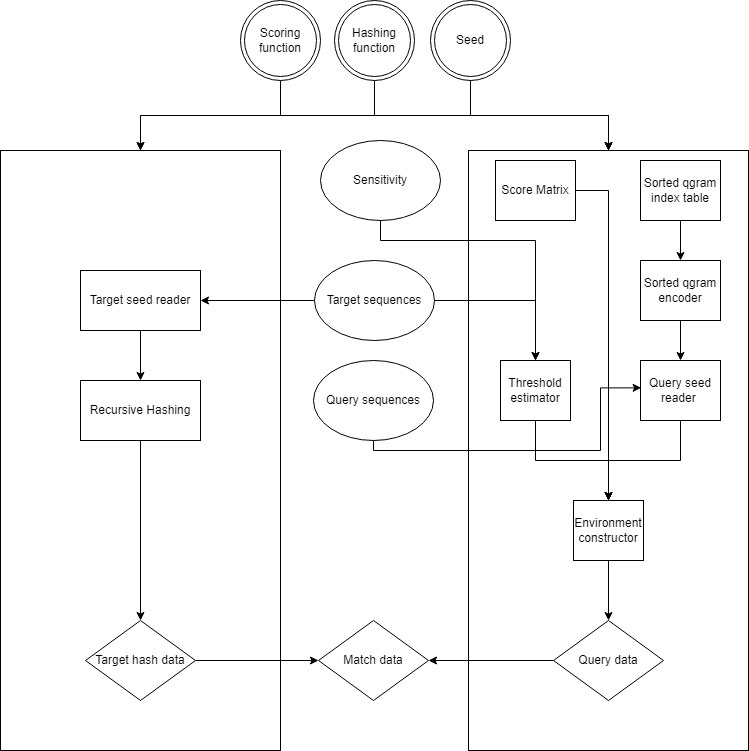
\includegraphics[scale=0.5]{graphics/Class_Diagram.png}
\end{center}
\caption{Relationship between the main classes and inputs}
\label{fig:classes}
\end{figure}